\documentclass[1p]{elsarticle_modified}
%\bibliographystyle{elsarticle-num}

%\usepackage[colorlinks]{hyperref}
%\usepackage{abbrmath_seonhwa} %\Abb, \Ascr, \Acal ,\Abf, \Afrak
\usepackage{amsfonts}
\usepackage{amssymb}
\usepackage{amsmath}
\usepackage{amsthm}
\usepackage{scalefnt}
\usepackage{amsbsy}
\usepackage{kotex}
\usepackage{caption}
\usepackage{subfig}
\usepackage{color}
\usepackage{graphicx}
\usepackage{xcolor} %% white, black, red, green, blue, cyan, magenta, yellow
\usepackage{float}
\usepackage{setspace}
\usepackage{hyperref}

\usepackage{tikz}
\usetikzlibrary{arrows}

\usepackage{multirow}
\usepackage{array} % fixed length table
\usepackage{hhline}

%%%%%%%%%%%%%%%%%%%%%
\makeatletter
\renewcommand*\env@matrix[1][\arraystretch]{%
	\edef\arraystretch{#1}%
	\hskip -\arraycolsep
	\let\@ifnextchar\new@ifnextchar
	\array{*\c@MaxMatrixCols c}}
\makeatother %https://tex.stackexchange.com/questions/14071/how-can-i-increase-the-line-spacing-in-a-matrix
%%%%%%%%%%%%%%%

\usepackage[normalem]{ulem}

\newcommand{\msout}[1]{\ifmmode\text{\sout{\ensuremath{#1}}}\else\sout{#1}\fi}
%SOURCE: \msout is \stkout macro in https://tex.stackexchange.com/questions/20609/strikeout-in-math-mode

\newcommand{\cancel}[1]{
	\ifmmode
	{\color{red}\msout{#1}}
	\else
	{\color{red}\sout{#1}}
	\fi
}

\newcommand{\add}[1]{
	{\color{blue}\uwave{#1}}
}

\newcommand{\replace}[2]{
	\ifmmode
	{\color{red}\msout{#1}}{\color{blue}\uwave{#2}}
	\else
	{\color{red}\sout{#1}}{\color{blue}\uwave{#2}}
	\fi
}

\newcommand{\Sol}{\mathcal{S}} %segment
\newcommand{\D}{D} %diagram
\newcommand{\A}{\mathcal{A}} %arc


%%%%%%%%%%%%%%%%%%%%%%%%%%%%%5 test

\def\sl{\operatorname{\textup{SL}}(2,\Cbb)}
\def\psl{\operatorname{\textup{PSL}}(2,\Cbb)}
\def\quan{\mkern 1mu \triangleright \mkern 1mu}

\theoremstyle{definition}
\newtheorem{thm}{Theorem}[section]
\newtheorem{prop}[thm]{Proposition}
\newtheorem{lem}[thm]{Lemma}
\newtheorem{ques}[thm]{Question}
\newtheorem{cor}[thm]{Corollary}
\newtheorem{defn}[thm]{Definition}
\newtheorem{exam}[thm]{Example}
\newtheorem{rmk}[thm]{Remark}
\newtheorem{alg}[thm]{Algorithm}

\newcommand{\I}{\sqrt{-1}}
\begin{document}

%\begin{frontmatter}
%
%\title{Boundary parabolic representations of knots up to 8 crossings}
%
%%% Group authors per affiliation:
%\author{Yunhi Cho} 
%\address{Department of Mathematics, University of Seoul, Seoul, Korea}
%\ead{yhcho@uos.ac.kr}
%
%
%\author{Seonhwa Kim} %\fnref{s_kim}}
%\address{Center for Geometry and Physics, Institute for Basic Science, Pohang, 37673, Korea}
%\ead{ryeona17@ibs.re.kr}
%
%\author{Hyuk Kim}
%\address{Department of Mathematical Sciences, Seoul National University, Seoul 08826, Korea}
%\ead{hyukkim@snu.ac.kr}
%
%\author{Seokbeom Yoon}
%\address{Department of Mathematical Sciences, Seoul National University, Seoul, 08826,  Korea}
%\ead{sbyoon15@snu.ac.kr}
%
%\begin{abstract}
%We find all boundary parabolic representation of knots up to 8 crossings.
%
%\end{abstract}
%\begin{keyword}
%    \MSC[2010] 57M25 
%\end{keyword}
%
%\end{frontmatter}

%\linenumbers
%\tableofcontents
%
\newcommand\colored[1]{\textcolor{white}{\rule[-0.35ex]{0.8em}{1.4ex}}\kern-0.8em\color{red} #1}%
%\newcommand\colored[1]{\textcolor{white}{ #1}\kern-2.17ex	\textcolor{white}{ #1}\kern-1.81ex	\textcolor{white}{ #1}\kern-2.15ex\color{red}#1	}

{\Large $\underline{12a_{0608}~(K12a_{0608})}$}

\setlength{\tabcolsep}{10pt}
\renewcommand{\arraystretch}{1.6}
\vspace{1cm}\begin{tabular}{m{100pt}>{\centering\arraybackslash}m{274pt}}
\multirow{5}{120pt}{
	\centering
	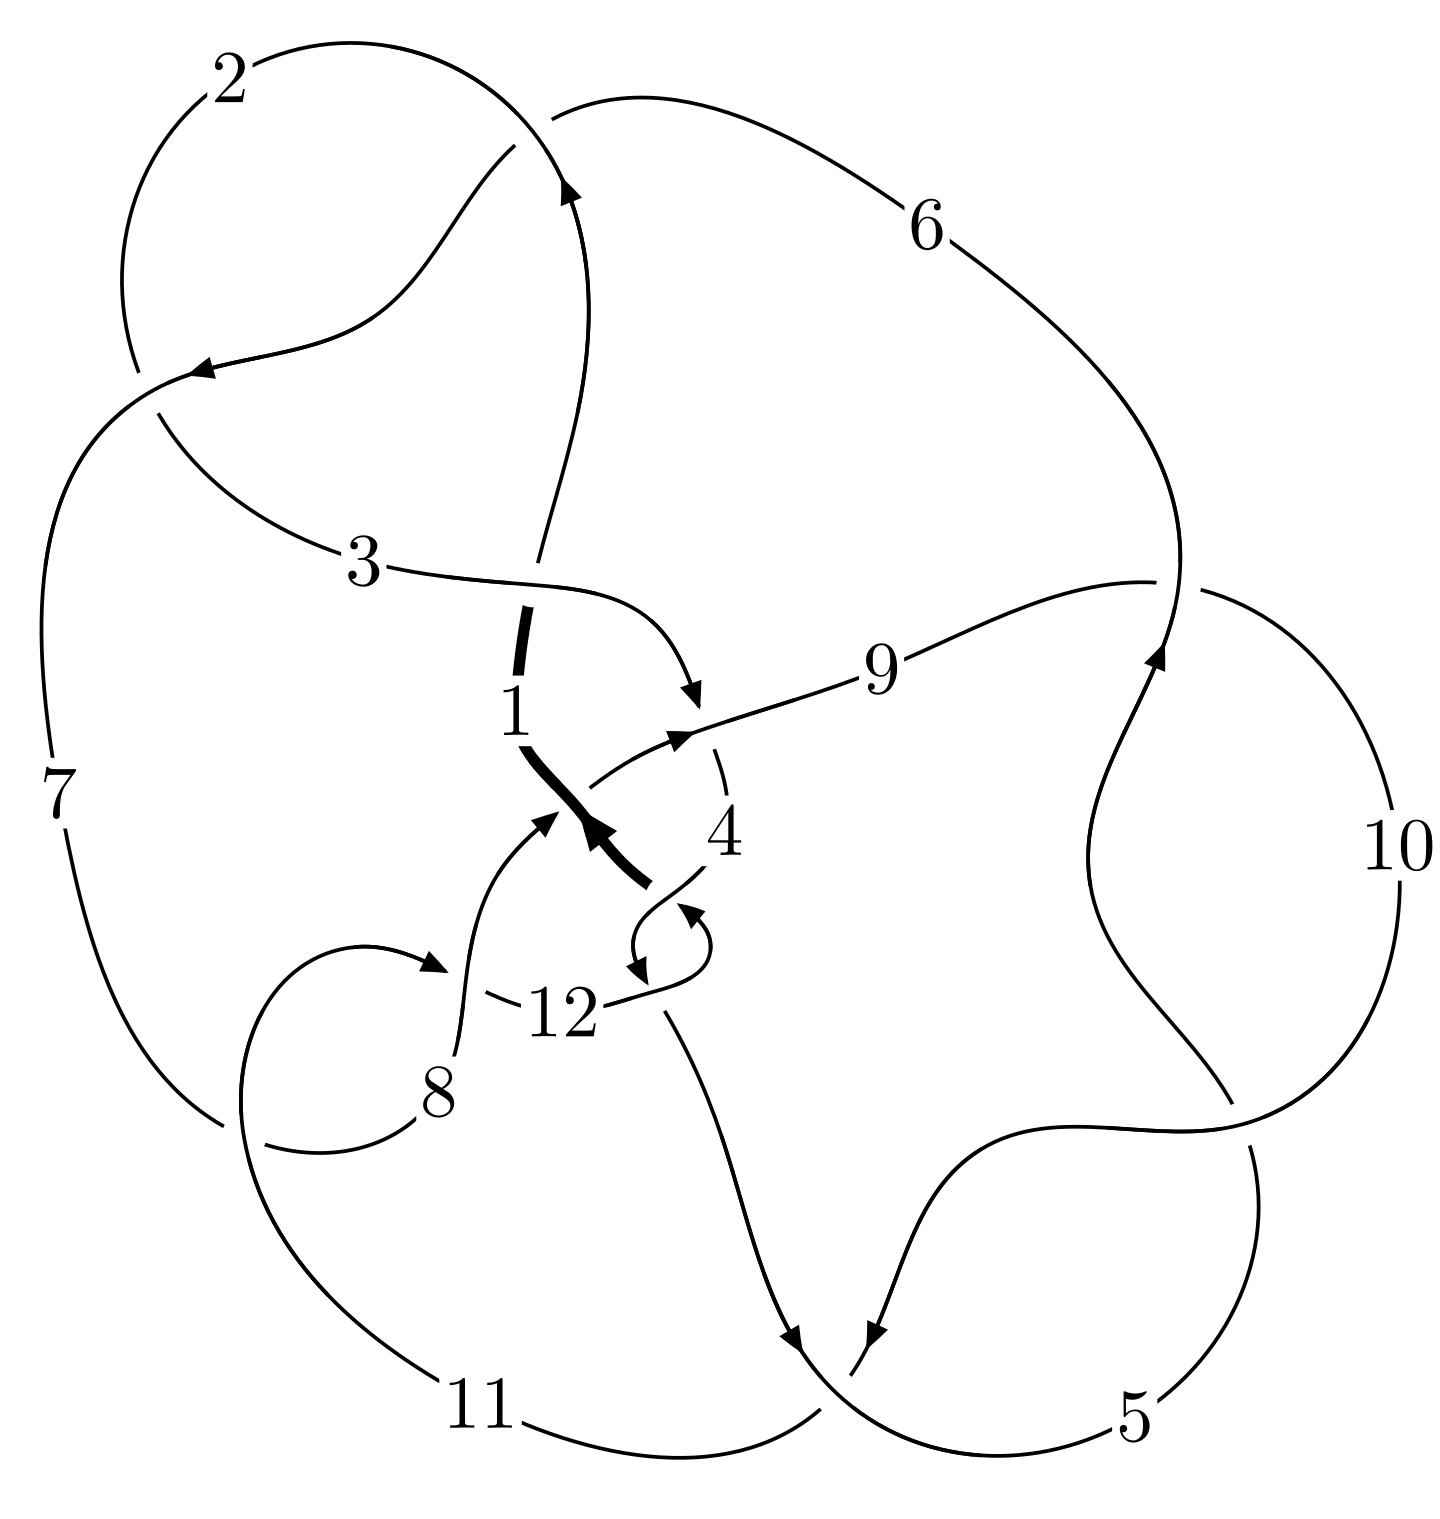
\includegraphics[width=112pt]{../../../GIT/diagram.site/Diagrams/png/1409_12a_0608.png}\\
\ \ \ A knot diagram\footnotemark}&
\allowdisplaybreaks
\textbf{Linearized knot diagam} \\
\cline{2-2}
 &
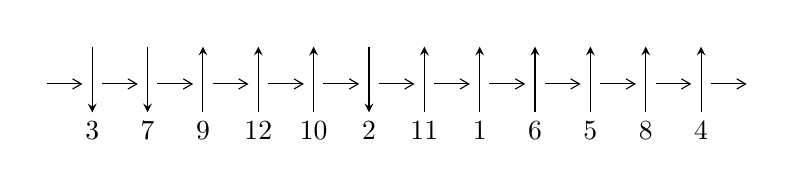
\begin{tikzpicture}[x=20pt, y=17pt]
	% nodes
	\node (C0) at (0, 0) {};
	\node (C1) at (1, 0) {};
	\node (C1U) at (1, +1) {};
	\node (C1D) at (1, -1) {3};

	\node (C2) at (2, 0) {};
	\node (C2U) at (2, +1) {};
	\node (C2D) at (2, -1) {7};

	\node (C3) at (3, 0) {};
	\node (C3U) at (3, +1) {};
	\node (C3D) at (3, -1) {9};

	\node (C4) at (4, 0) {};
	\node (C4U) at (4, +1) {};
	\node (C4D) at (4, -1) {12};

	\node (C5) at (5, 0) {};
	\node (C5U) at (5, +1) {};
	\node (C5D) at (5, -1) {10};

	\node (C6) at (6, 0) {};
	\node (C6U) at (6, +1) {};
	\node (C6D) at (6, -1) {2};

	\node (C7) at (7, 0) {};
	\node (C7U) at (7, +1) {};
	\node (C7D) at (7, -1) {11};

	\node (C8) at (8, 0) {};
	\node (C8U) at (8, +1) {};
	\node (C8D) at (8, -1) {1};

	\node (C9) at (9, 0) {};
	\node (C9U) at (9, +1) {};
	\node (C9D) at (9, -1) {6};

	\node (C10) at (10, 0) {};
	\node (C10U) at (10, +1) {};
	\node (C10D) at (10, -1) {5};

	\node (C11) at (11, 0) {};
	\node (C11U) at (11, +1) {};
	\node (C11D) at (11, -1) {8};

	\node (C12) at (12, 0) {};
	\node (C12U) at (12, +1) {};
	\node (C12D) at (12, -1) {4};
	\node (C13) at (13, 0) {};

	% arrows
	\draw[->,>={angle 60}]
	(C0) edge (C1) (C1) edge (C2) (C2) edge (C3) (C3) edge (C4) (C4) edge (C5) (C5) edge (C6) (C6) edge (C7) (C7) edge (C8) (C8) edge (C9) (C9) edge (C10) (C10) edge (C11) (C11) edge (C12) (C12) edge (C13) ;	\draw[->,>=stealth]
	(C1U) edge (C1D) (C2U) edge (C2D) (C3D) edge (C3U) (C4D) edge (C4U) (C5D) edge (C5U) (C6U) edge (C6D) (C7D) edge (C7U) (C8D) edge (C8U) (C9D) edge (C9U) (C10D) edge (C10U) (C11D) edge (C11U) (C12D) edge (C12U) ;
	\end{tikzpicture} \\
\hhline{~~} \\& 
\textbf{Solving Sequence} \\ \cline{2-2} 
 &
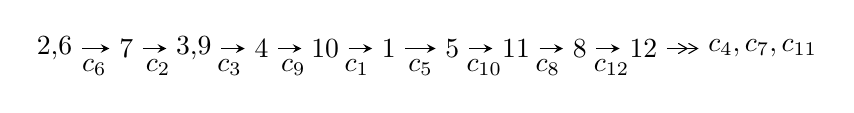
\begin{tikzpicture}[x=23pt, y=7pt]
	% node
	\node (A0) at (-1/8, 0) {2,6};
	\node (A1) at (1, 0) {7};
	\node (A2) at (33/16, 0) {3,9};
	\node (A3) at (25/8, 0) {4};
	\node (A4) at (33/8, 0) {10};
	\node (A5) at (41/8, 0) {1};
	\node (A6) at (49/8, 0) {5};
	\node (A7) at (57/8, 0) {11};
	\node (A8) at (65/8, 0) {8};
	\node (A9) at (73/8, 0) {12};
	\node (C1) at (1/2, -1) {$c_{6}$};
	\node (C2) at (3/2, -1) {$c_{2}$};
	\node (C3) at (21/8, -1) {$c_{3}$};
	\node (C4) at (29/8, -1) {$c_{9}$};
	\node (C5) at (37/8, -1) {$c_{1}$};
	\node (C6) at (45/8, -1) {$c_{5}$};
	\node (C7) at (53/8, -1) {$c_{10}$};
	\node (C8) at (61/8, -1) {$c_{8}$};
	\node (C9) at (69/8, -1) {$c_{12}$};
	\node (A10) at (11, 0) {$c_{4},c_{7},c_{11}$};

	% edge
	\draw[->,>=stealth]	
	(A0) edge (A1) (A1) edge (A2) (A2) edge (A3) (A3) edge (A4) (A4) edge (A5) (A5) edge (A6) (A6) edge (A7) (A7) edge (A8) (A8) edge (A9) ;
	\draw[->>,>={angle 60}]	
	(A9) edge (A10);
\end{tikzpicture} \\ 

\end{tabular} \\

\footnotetext{
The image of knot diagram is generated by the software ``\textbf{Draw programme}" developed by Andrew Bartholomew(\url{http://www.layer8.co.uk/maths/draw/index.htm\#Running-draw}), where we modified some parts for our purpose(\url{https://github.com/CATsTAILs/LinksPainter}).
}\phantom \\ \newline 
\centering \textbf{Ideals for irreducible components\footnotemark of $X_{\text{par}}$} 
 
\begin{align*}
I^u_{1}&=\langle 
-1.91359\times10^{294} u^{122}-4.52981\times10^{294} u^{121}+\cdots+3.88967\times10^{294} b-2.98604\times10^{296},\\
\phantom{I^u_{1}}&\phantom{= \langle  }-9.79728\times10^{295} u^{122}-2.24169\times10^{296} u^{121}+\cdots+4.00636\times10^{296} a-7.79915\times10^{297},\\
\phantom{I^u_{1}}&\phantom{= \langle  }u^{123}+3 u^{122}+\cdots+118 u+103\rangle \\
I^u_{2}&=\langle 
88 u^{27}+45 u^{26}+\cdots+23 b-99,\;-10 u^{27}+78 u^{26}+\cdots+23 a-144,\;u^{28}-7 u^{26}+\cdots-8 u^2+1\rangle \\
\\
\end{align*}
\raggedright * 2 irreducible components of $\dim_{\mathbb{C}}=0$, with total 151 representations.\\
\footnotetext{All coefficients of polynomials are rational numbers. But the coefficients are sometimes approximated in decimal forms when there is not enough margin.}
\newpage
\renewcommand{\arraystretch}{1}
\centering \section*{I. $I^u_{1}= \langle -1.91\times10^{294} u^{122}-4.53\times10^{294} u^{121}+\cdots+3.89\times10^{294} b-2.99\times10^{296},\;-9.80\times10^{295} u^{122}-2.24\times10^{296} u^{121}+\cdots+4.01\times10^{296} a-7.80\times10^{297},\;u^{123}+3 u^{122}+\cdots+118 u+103 \rangle$}
\flushleft \textbf{(i) Arc colorings}\\
\begin{tabular}{m{7pt} m{180pt} m{7pt} m{180pt} }
\flushright $a_{2}=$&$\begin{pmatrix}0\\u\end{pmatrix}$ \\
\flushright $a_{6}=$&$\begin{pmatrix}1\\0\end{pmatrix}$ \\
\flushright $a_{7}=$&$\begin{pmatrix}1\\u^2\end{pmatrix}$ \\
\flushright $a_{3}=$&$\begin{pmatrix}- u\\- u^3+u\end{pmatrix}$ \\
\flushright $a_{9}=$&$\begin{pmatrix}0.244543 u^{122}+0.559534 u^{121}+\cdots-28.9145 u+19.4669\\0.491968 u^{122}+1.16457 u^{121}+\cdots+4.25457 u+76.7685\end{pmatrix}$ \\
\flushright $a_{4}=$&$\begin{pmatrix}-1.06929 u^{122}-2.35492 u^{121}+\cdots-11.6245 u-175.307\\-0.153231 u^{122}-0.387862 u^{121}+\cdots+11.1290 u-2.47162\end{pmatrix}$ \\
\flushright $a_{10}=$&$\begin{pmatrix}0.736511 u^{122}+1.72411 u^{121}+\cdots-24.6599 u+96.2354\\0.491968 u^{122}+1.16457 u^{121}+\cdots+4.25457 u+76.7685\end{pmatrix}$ \\
\flushright $a_{1}=$&$\begin{pmatrix}u^3\\u^5- u^3+u\end{pmatrix}$ \\
\flushright $a_{5}=$&$\begin{pmatrix}0.415775 u^{122}+0.783733 u^{121}+\cdots+11.3829 u+77.3969\\-0.364639 u^{122}-0.941621 u^{121}+\cdots+18.7141 u-45.2372\end{pmatrix}$ \\
\flushright $a_{11}=$&$\begin{pmatrix}0.366534 u^{122}+0.922878 u^{121}+\cdots-25.4284 u+50.5634\\0.319860 u^{122}+0.705880 u^{121}+\cdots-17.4424 u+46.0162\end{pmatrix}$ \\
\flushright $a_{8}=$&$\begin{pmatrix}0.408604 u^{122}+0.923887 u^{121}+\cdots-20.1527 u+36.3808\\0.573783 u^{122}+1.34367 u^{121}+\cdots+3.16407 u+79.2098\end{pmatrix}$ \\
\flushright $a_{12}=$&$\begin{pmatrix}0.168150 u^{122}+0.451184 u^{121}+\cdots+10.0432 u+61.5193\\0.0421304 u^{122}+0.0512572 u^{121}+\cdots+8.54951 u+21.5981\end{pmatrix}$\\&\end{tabular}
\flushleft \textbf{(ii) Obstruction class $= -1$}\\~\\
\flushleft \textbf{(iii) Cusp Shapes $= 0.0861323 u^{122}+0.301447 u^{121}+\cdots-68.2666 u+155.020$}\\~\\
\newpage\renewcommand{\arraystretch}{1}
\flushleft \textbf{(iv) u-Polynomials at the component}\newline \\
\begin{tabular}{m{50pt}|m{274pt}}
Crossings & \hspace{64pt}u-Polynomials at each crossing \\
\hline $$\begin{aligned}c_{1}\end{aligned}$$&$\begin{aligned}
&u^{123}+55 u^{122}+\cdots+363300 u+10609
\end{aligned}$\\
\hline $$\begin{aligned}c_{2},c_{6}\end{aligned}$$&$\begin{aligned}
&u^{123}-3 u^{122}+\cdots+118 u-103
\end{aligned}$\\
\hline $$\begin{aligned}c_{3}\end{aligned}$$&$\begin{aligned}
&u^{123}- u^{122}+\cdots+87046 u-12899
\end{aligned}$\\
\hline $$\begin{aligned}c_{4},c_{12}\end{aligned}$$&$\begin{aligned}
&u^{123}+7 u^{122}+\cdots-111 u-43
\end{aligned}$\\
\hline $$\begin{aligned}c_{5},c_{9},c_{10}\end{aligned}$$&$\begin{aligned}
&u^{123}- u^{122}+\cdots+u-19
\end{aligned}$\\
\hline $$\begin{aligned}c_{7},c_{11}\end{aligned}$$&$\begin{aligned}
&u^{123}+3 u^{122}+\cdots-752 u-187
\end{aligned}$\\
\hline $$\begin{aligned}c_{8}\end{aligned}$$&$\begin{aligned}
&u^{123}+2 u^{122}+\cdots+2 u-1
\end{aligned}$\\
\hline
\end{tabular}\\~\\
\newpage\renewcommand{\arraystretch}{1}
\flushleft \textbf{(v) Riley Polynomials at the component}\newline \\
\begin{tabular}{m{50pt}|m{274pt}}
Crossings & \hspace{64pt}Riley Polynomials at each crossing \\
\hline $$\begin{aligned}c_{1}\end{aligned}$$&$\begin{aligned}
&y^{123}+41 y^{122}+\cdots+2225325352 y-112550881
\end{aligned}$\\
\hline $$\begin{aligned}c_{2},c_{6}\end{aligned}$$&$\begin{aligned}
&y^{123}-55 y^{122}+\cdots+363300 y-10609
\end{aligned}$\\
\hline $$\begin{aligned}c_{3}\end{aligned}$$&$\begin{aligned}
&y^{123}+27 y^{122}+\cdots-6188058542 y-166384201
\end{aligned}$\\
\hline $$\begin{aligned}c_{4},c_{12}\end{aligned}$$&$\begin{aligned}
&y^{123}+91 y^{122}+\cdots-18639 y-1849
\end{aligned}$\\
\hline $$\begin{aligned}c_{5},c_{9},c_{10}\end{aligned}$$&$\begin{aligned}
&y^{123}+123 y^{122}+\cdots-47879 y-361
\end{aligned}$\\
\hline $$\begin{aligned}c_{7},c_{11}\end{aligned}$$&$\begin{aligned}
&y^{123}-69 y^{122}+\cdots+1826632 y-34969
\end{aligned}$\\
\hline $$\begin{aligned}c_{8}\end{aligned}$$&$\begin{aligned}
&y^{123}-10 y^{122}+\cdots+136 y-1
\end{aligned}$\\
\hline
\end{tabular}\\~\\
\newpage\flushleft \textbf{(vi) Complex Volumes and Cusp Shapes}
$$\begin{array}{c|c|c}  
\text{Solutions to }I^u_{1}& \I (\text{vol} + \sqrt{-1}CS) & \text{Cusp shape}\\
 \hline 
\begin{aligned}
u &= -0.787312 + 0.611782 I \\
a &= \phantom{-}1.347980 - 0.063462 I \\
b &= -0.704765 + 0.157248 I\end{aligned}
 & \phantom{-}2.06112 - 0.67907 I & \phantom{-0.000000 } 0 \\ \hline\begin{aligned}
u &= -0.787312 - 0.611782 I \\
a &= \phantom{-}1.347980 + 0.063462 I \\
b &= -0.704765 - 0.157248 I\end{aligned}
 & \phantom{-}2.06112 + 0.67907 I & \phantom{-0.000000 } 0 \\ \hline\begin{aligned}
u &= \phantom{-}0.948530 + 0.334543 I \\
a &= \phantom{-}1.52357 + 0.72529 I \\
b &= -1.032510 + 0.448117 I\end{aligned}
 & -2.63821 + 1.05482 I & \phantom{-0.000000 } 0 \\ \hline\begin{aligned}
u &= \phantom{-}0.948530 - 0.334543 I \\
a &= \phantom{-}1.52357 - 0.72529 I \\
b &= -1.032510 - 0.448117 I\end{aligned}
 & -2.63821 - 1.05482 I & \phantom{-0.000000 } 0 \\ \hline\begin{aligned}
u &= \phantom{-}0.407053 + 0.920884 I \\
a &= -0.282292 + 0.316166 I \\
b &= \phantom{-}0.397219 - 0.046853 I\end{aligned}
 & \phantom{-}1.20818 - 4.13474 I & \phantom{-0.000000 } 0 \\ \hline\begin{aligned}
u &= \phantom{-}0.407053 - 0.920884 I \\
a &= -0.282292 - 0.316166 I \\
b &= \phantom{-}0.397219 + 0.046853 I\end{aligned}
 & \phantom{-}1.20818 + 4.13474 I & \phantom{-0.000000 } 0 \\ \hline\begin{aligned}
u &= -0.515334 + 0.875291 I \\
a &= \phantom{-}0.506060 - 1.177120 I \\
b &= -0.15168 + 1.45970 I\end{aligned}
 & -7.77774 - 4.96669 I & \phantom{-0.000000 } 0 \\ \hline\begin{aligned}
u &= -0.515334 - 0.875291 I \\
a &= \phantom{-}0.506060 + 1.177120 I \\
b &= -0.15168 - 1.45970 I\end{aligned}
 & -7.77774 + 4.96669 I & \phantom{-0.000000 } 0 \\ \hline\begin{aligned}
u &= \phantom{-}0.742368 + 0.694050 I \\
a &= -1.144460 - 0.407527 I \\
b &= \phantom{-}0.473434 - 0.779230 I\end{aligned}
 & \phantom{-}4.20707 - 2.00630 I & \phantom{-0.000000 } 0 \\ \hline\begin{aligned}
u &= \phantom{-}0.742368 - 0.694050 I \\
a &= -1.144460 + 0.407527 I \\
b &= \phantom{-}0.473434 + 0.779230 I\end{aligned}
 & \phantom{-}4.20707 + 2.00630 I & \phantom{-0.000000 } 0\\
 \hline 
 \end{array}$$\newpage$$\begin{array}{c|c|c}  
\text{Solutions to }I^u_{1}& \I (\text{vol} + \sqrt{-1}CS) & \text{Cusp shape}\\
 \hline 
\begin{aligned}
u &= \phantom{-}0.899456 + 0.386524 I \\
a &= -1.205040 - 0.331370 I \\
b &= -0.07659 - 1.90314 I\end{aligned}
 & -11.55850 - 1.59415 I & \phantom{-0.000000 } 0 \\ \hline\begin{aligned}
u &= \phantom{-}0.899456 - 0.386524 I \\
a &= -1.205040 + 0.331370 I \\
b &= -0.07659 + 1.90314 I\end{aligned}
 & -11.55850 + 1.59415 I & \phantom{-0.000000 } 0 \\ \hline\begin{aligned}
u &= -0.940419 + 0.400277 I \\
a &= \phantom{-}2.58071 - 1.55175 I \\
b &= \phantom{-}0.022898 - 1.315310 I\end{aligned}
 & -4.61342 - 3.20939 I & \phantom{-0.000000 } 0 \\ \hline\begin{aligned}
u &= -0.940419 - 0.400277 I \\
a &= \phantom{-}2.58071 + 1.55175 I \\
b &= \phantom{-}0.022898 + 1.315310 I\end{aligned}
 & -4.61342 + 3.20939 I & \phantom{-0.000000 } 0 \\ \hline\begin{aligned}
u &= -0.547983 + 0.864160 I \\
a &= -0.831442 + 0.465828 I \\
b &= \phantom{-}0.716478 - 0.312874 I\end{aligned}
 & \phantom{-}5.66260 - 2.23601 I & \phantom{-0.000000 } 0 \\ \hline\begin{aligned}
u &= -0.547983 - 0.864160 I \\
a &= -0.831442 - 0.465828 I \\
b &= \phantom{-}0.716478 + 0.312874 I\end{aligned}
 & \phantom{-}5.66260 + 2.23601 I & \phantom{-0.000000 } 0 \\ \hline\begin{aligned}
u &= \phantom{-}0.499148 + 0.825004 I \\
a &= -1.173990 - 0.748238 I \\
b &= \phantom{-}0.899665 + 0.392483 I\end{aligned}
 & \phantom{-}1.63268 + 7.95122 I & \phantom{-0.000000 } 0 \\ \hline\begin{aligned}
u &= \phantom{-}0.499148 - 0.825004 I \\
a &= -1.173990 + 0.748238 I \\
b &= \phantom{-}0.899665 - 0.392483 I\end{aligned}
 & \phantom{-}1.63268 - 7.95122 I & \phantom{-0.000000 } 0 \\ \hline\begin{aligned}
u &= \phantom{-}1.003890 + 0.321587 I \\
a &= -0.164326 - 0.143765 I \\
b &= \phantom{-}0.175029 + 0.466402 I\end{aligned}
 & -1.66108 - 1.47407 I & \phantom{-0.000000 } 0 \\ \hline\begin{aligned}
u &= \phantom{-}1.003890 - 0.321587 I \\
a &= -0.164326 + 0.143765 I \\
b &= \phantom{-}0.175029 - 0.466402 I\end{aligned}
 & -1.66108 + 1.47407 I & \phantom{-0.000000 } 0\\
 \hline 
 \end{array}$$\newpage$$\begin{array}{c|c|c}  
\text{Solutions to }I^u_{1}& \I (\text{vol} + \sqrt{-1}CS) & \text{Cusp shape}\\
 \hline 
\begin{aligned}
u &= -1.042520 + 0.171631 I \\
a &= -0.238632 - 0.296052 I \\
b &= \phantom{-}0.433016 - 0.822238 I\end{aligned}
 & -5.79252 - 1.16404 I & \phantom{-0.000000 } 0 \\ \hline\begin{aligned}
u &= -1.042520 - 0.171631 I \\
a &= -0.238632 + 0.296052 I \\
b &= \phantom{-}0.433016 + 0.822238 I\end{aligned}
 & -5.79252 + 1.16404 I & \phantom{-0.000000 } 0 \\ \hline\begin{aligned}
u &= -0.945639 + 0.472768 I \\
a &= -1.54105 + 1.40262 I \\
b &= \phantom{-}0.13061 + 1.51319 I\end{aligned}
 & -3.11222 + 3.71000 I & \phantom{-0.000000 } 0 \\ \hline\begin{aligned}
u &= -0.945639 - 0.472768 I \\
a &= -1.54105 - 1.40262 I \\
b &= \phantom{-}0.13061 - 1.51319 I\end{aligned}
 & -3.11222 - 3.71000 I & \phantom{-0.000000 } 0 \\ \hline\begin{aligned}
u &= -1.068950 + 0.027148 I \\
a &= -0.065840 + 0.370856 I \\
b &= -0.516622 - 0.708624 I\end{aligned}
 & -4.17554 + 6.43085 I & \phantom{-0.000000 } 0 \\ \hline\begin{aligned}
u &= -1.068950 - 0.027148 I \\
a &= -0.065840 - 0.370856 I \\
b &= -0.516622 + 0.708624 I\end{aligned}
 & -4.17554 - 6.43085 I & \phantom{-0.000000 } 0 \\ \hline\begin{aligned}
u &= \phantom{-}0.964494 + 0.465733 I \\
a &= \phantom{-}2.41393 + 0.37226 I \\
b &= -0.089867 + 1.348840 I\end{aligned}
 & -3.08837 - 1.58092 I & \phantom{-0.000000 } 0 \\ \hline\begin{aligned}
u &= \phantom{-}0.964494 - 0.465733 I \\
a &= \phantom{-}2.41393 - 0.37226 I \\
b &= -0.089867 - 1.348840 I\end{aligned}
 & -3.08837 + 1.58092 I & \phantom{-0.000000 } 0 \\ \hline\begin{aligned}
u &= -0.875483 + 0.638970 I \\
a &= -1.16011 + 1.11661 I \\
b &= \phantom{-}0.585032 + 0.257556 I\end{aligned}
 & \phantom{-}1.80755 + 5.59259 I & \phantom{-0.000000 } 0 \\ \hline\begin{aligned}
u &= -0.875483 - 0.638970 I \\
a &= -1.16011 - 1.11661 I \\
b &= \phantom{-}0.585032 - 0.257556 I\end{aligned}
 & \phantom{-}1.80755 - 5.59259 I & \phantom{-0.000000 } 0\\
 \hline 
 \end{array}$$\newpage$$\begin{array}{c|c|c}  
\text{Solutions to }I^u_{1}& \I (\text{vol} + \sqrt{-1}CS) & \text{Cusp shape}\\
 \hline 
\begin{aligned}
u &= -0.437385 + 0.992590 I \\
a &= -0.508035 + 0.885387 I \\
b &= \phantom{-}0.33220 - 1.49038 I\end{aligned}
 & -4.42863 - 12.37890 I & \phantom{-0.000000 } 0 \\ \hline\begin{aligned}
u &= -0.437385 - 0.992590 I \\
a &= -0.508035 - 0.885387 I \\
b &= \phantom{-}0.33220 + 1.49038 I\end{aligned}
 & -4.42863 + 12.37890 I & \phantom{-0.000000 } 0 \\ \hline\begin{aligned}
u &= \phantom{-}1.029890 + 0.363744 I \\
a &= -0.735917 - 0.877515 I \\
b &= \phantom{-}1.005630 - 0.051546 I\end{aligned}
 & -2.96783 - 3.24228 I & \phantom{-0.000000 } 0 \\ \hline\begin{aligned}
u &= \phantom{-}1.029890 - 0.363744 I \\
a &= -0.735917 + 0.877515 I \\
b &= \phantom{-}1.005630 + 0.051546 I\end{aligned}
 & -2.96783 + 3.24228 I & \phantom{-0.000000 } 0 \\ \hline\begin{aligned}
u &= -0.859174 + 0.266582 I \\
a &= -0.864643 + 1.047260 I \\
b &= -0.122746 - 1.028840 I\end{aligned}
 & -4.11003 + 6.16993 I & \phantom{-0.000000 } 0 \\ \hline\begin{aligned}
u &= -0.859174 - 0.266582 I \\
a &= -0.864643 - 1.047260 I \\
b &= -0.122746 + 1.028840 I\end{aligned}
 & -4.11003 - 6.16993 I & \phantom{-0.000000 } 0 \\ \hline\begin{aligned}
u &= \phantom{-}0.866442 + 0.686571 I \\
a &= \phantom{-}0.021204 - 0.798522 I \\
b &= -0.082816 - 0.345180 I\end{aligned}
 & \phantom{-}3.81153 - 2.64755 I & \phantom{-0.000000 } 0 \\ \hline\begin{aligned}
u &= \phantom{-}0.866442 - 0.686571 I \\
a &= \phantom{-}0.021204 + 0.798522 I \\
b &= -0.082816 + 0.345180 I\end{aligned}
 & \phantom{-}3.81153 + 2.64755 I & \phantom{-0.000000 } 0 \\ \hline\begin{aligned}
u &= -0.457246 + 0.766444 I \\
a &= \phantom{-}0.295154 + 1.361580 I \\
b &= \phantom{-}0.10777 - 1.49701 I\end{aligned}
 & -8.07051 + 1.26448 I & \phantom{-0.000000 } 0 \\ \hline\begin{aligned}
u &= -0.457246 - 0.766444 I \\
a &= \phantom{-}0.295154 - 1.361580 I \\
b &= \phantom{-}0.10777 + 1.49701 I\end{aligned}
 & -8.07051 - 1.26448 I & \phantom{-0.000000 } 0\\
 \hline 
 \end{array}$$\newpage$$\begin{array}{c|c|c}  
\text{Solutions to }I^u_{1}& \I (\text{vol} + \sqrt{-1}CS) & \text{Cusp shape}\\
 \hline 
\begin{aligned}
u &= -0.782458 + 0.421266 I \\
a &= \phantom{-}0.492123 + 0.259294 I \\
b &= -0.25826 + 1.42214 I\end{aligned}
 & -2.49887 + 0.02070 I & \phantom{-0.000000 } 0 \\ \hline\begin{aligned}
u &= -0.782458 - 0.421266 I \\
a &= \phantom{-}0.492123 - 0.259294 I \\
b &= -0.25826 - 1.42214 I\end{aligned}
 & -2.49887 - 0.02070 I & \phantom{-0.000000 } 0 \\ \hline\begin{aligned}
u &= \phantom{-}0.923397 + 0.629238 I \\
a &= \phantom{-}0.459018 + 0.164260 I \\
b &= -0.621856 - 0.578750 I\end{aligned}
 & \phantom{-}3.64481 - 3.09137 I & \phantom{-0.000000 } 0 \\ \hline\begin{aligned}
u &= \phantom{-}0.923397 - 0.629238 I \\
a &= \phantom{-}0.459018 - 0.164260 I \\
b &= -0.621856 + 0.578750 I\end{aligned}
 & \phantom{-}3.64481 + 3.09137 I & \phantom{-0.000000 } 0 \\ \hline\begin{aligned}
u &= \phantom{-}0.980910 + 0.535352 I \\
a &= -2.34185 - 1.18607 I \\
b &= \phantom{-}0.22577 - 1.42603 I\end{aligned}
 & -3.65229 - 8.55997 I & \phantom{-0.000000 } 0 \\ \hline\begin{aligned}
u &= \phantom{-}0.980910 - 0.535352 I \\
a &= -2.34185 + 1.18607 I \\
b &= \phantom{-}0.22577 + 1.42603 I\end{aligned}
 & -3.65229 + 8.55997 I & \phantom{-0.000000 } 0 \\ \hline\begin{aligned}
u &= \phantom{-}0.385592 + 1.050480 I \\
a &= -0.281760 - 0.585327 I \\
b &= \phantom{-}0.24772 + 1.43250 I\end{aligned}
 & \phantom{-}0.06289 + 5.69076 I & \phantom{-0.000000 } 0 \\ \hline\begin{aligned}
u &= \phantom{-}0.385592 - 1.050480 I \\
a &= -0.281760 + 0.585327 I \\
b &= \phantom{-}0.24772 - 1.43250 I\end{aligned}
 & \phantom{-}0.06289 - 5.69076 I & \phantom{-0.000000 } 0 \\ \hline\begin{aligned}
u &= \phantom{-}0.169806 + 0.859437 I \\
a &= \phantom{-}0.524015 + 0.315294 I \\
b &= \phantom{-}0.018135 - 1.235180 I\end{aligned}
 & -2.18571 + 2.40188 I & \phantom{-0.000000 } 0 \\ \hline\begin{aligned}
u &= \phantom{-}0.169806 - 0.859437 I \\
a &= \phantom{-}0.524015 - 0.315294 I \\
b &= \phantom{-}0.018135 + 1.235180 I\end{aligned}
 & -2.18571 - 2.40188 I & \phantom{-0.000000 } 0\\
 \hline 
 \end{array}$$\newpage$$\begin{array}{c|c|c}  
\text{Solutions to }I^u_{1}& \I (\text{vol} + \sqrt{-1}CS) & \text{Cusp shape}\\
 \hline 
\begin{aligned}
u &= -1.003390 + 0.537040 I \\
a &= -1.171840 + 0.574067 I \\
b &= \phantom{-}0.616372 + 0.213805 I\end{aligned}
 & -0.26082 + 4.36982 I & \phantom{-0.000000 } 0 \\ \hline\begin{aligned}
u &= -1.003390 - 0.537040 I \\
a &= -1.171840 - 0.574067 I \\
b &= \phantom{-}0.616372 - 0.213805 I\end{aligned}
 & -0.26082 - 4.36982 I & \phantom{-0.000000 } 0 \\ \hline\begin{aligned}
u &= \phantom{-}0.660571 + 0.541819 I \\
a &= \phantom{-}1.171540 + 0.572811 I \\
b &= -0.270269 - 1.340010 I\end{aligned}
 & -2.63800 + 4.19479 I & \phantom{-0.000000 } 0 \\ \hline\begin{aligned}
u &= \phantom{-}0.660571 - 0.541819 I \\
a &= \phantom{-}1.171540 - 0.572811 I \\
b &= -0.270269 + 1.340010 I\end{aligned}
 & -2.63800 - 4.19479 I & \phantom{-0.000000 } 0 \\ \hline\begin{aligned}
u &= -1.005150 + 0.553399 I \\
a &= \phantom{-}0.353317 - 0.779011 I \\
b &= -1.022200 + 0.905486 I\end{aligned}
 & -1.13521 + 6.72211 I & \phantom{-0.000000 } 0 \\ \hline\begin{aligned}
u &= -1.005150 - 0.553399 I \\
a &= \phantom{-}0.353317 + 0.779011 I \\
b &= -1.022200 - 0.905486 I\end{aligned}
 & -1.13521 - 6.72211 I & \phantom{-0.000000 } 0 \\ \hline\begin{aligned}
u &= -1.114370 + 0.289346 I \\
a &= \phantom{-}0.331211 - 0.959738 I \\
b &= \phantom{-}0.160740 - 1.382660 I\end{aligned}
 & -6.91836 - 0.04737 I & \phantom{-0.000000 } 0 \\ \hline\begin{aligned}
u &= -1.114370 - 0.289346 I \\
a &= \phantom{-}0.331211 + 0.959738 I \\
b &= \phantom{-}0.160740 + 1.382660 I\end{aligned}
 & -6.91836 + 0.04737 I & \phantom{-0.000000 } 0 \\ \hline\begin{aligned}
u &= \phantom{-}0.889597 + 0.768873 I \\
a &= \phantom{-}0.626789 - 0.957771 I \\
b &= \phantom{-}0.043016 + 0.993124 I\end{aligned}
 & -0.21937 - 2.90174 I & \phantom{-0.000000 } 0 \\ \hline\begin{aligned}
u &= \phantom{-}0.889597 - 0.768873 I \\
a &= \phantom{-}0.626789 + 0.957771 I \\
b &= \phantom{-}0.043016 - 0.993124 I\end{aligned}
 & -0.21937 + 2.90174 I & \phantom{-0.000000 } 0\\
 \hline 
 \end{array}$$\newpage$$\begin{array}{c|c|c}  
\text{Solutions to }I^u_{1}& \I (\text{vol} + \sqrt{-1}CS) & \text{Cusp shape}\\
 \hline 
\begin{aligned}
u &= -0.602560 + 0.561546 I \\
a &= -2.00071 + 0.52026 I \\
b &= \phantom{-}0.795831 + 0.968113 I\end{aligned}
 & \phantom{-}0.10275 - 2.20920 I & \phantom{-0.000000 } 0 \\ \hline\begin{aligned}
u &= -0.602560 - 0.561546 I \\
a &= -2.00071 - 0.52026 I \\
b &= \phantom{-}0.795831 - 0.968113 I\end{aligned}
 & \phantom{-}0.10275 + 2.20920 I & \phantom{-0.000000 } 0 \\ \hline\begin{aligned}
u &= -1.074070 + 0.485368 I \\
a &= -0.610249 + 0.910638 I \\
b &= \phantom{-}0.924230 - 0.351363 I\end{aligned}
 & -2.13614 + 3.57490 I & \phantom{-0.000000 } 0 \\ \hline\begin{aligned}
u &= -1.074070 - 0.485368 I \\
a &= -0.610249 - 0.910638 I \\
b &= \phantom{-}0.924230 + 0.351363 I\end{aligned}
 & -2.13614 - 3.57490 I & \phantom{-0.000000 } 0 \\ \hline\begin{aligned}
u &= \phantom{-}0.639090 + 0.504053 I \\
a &= \phantom{-}1.077930 - 0.580036 I \\
b &= -0.192648 + 0.630385 I\end{aligned}
 & -0.71618 - 1.90859 I & \phantom{-0.000000 } 0 \\ \hline\begin{aligned}
u &= \phantom{-}0.639090 - 0.504053 I \\
a &= \phantom{-}1.077930 + 0.580036 I \\
b &= -0.192648 - 0.630385 I\end{aligned}
 & -0.71618 + 1.90859 I & \phantom{-0.000000 } 0 \\ \hline\begin{aligned}
u &= -1.045760 + 0.568872 I \\
a &= \phantom{-}1.73537 + 0.12208 I \\
b &= -0.25881 - 1.60054 I\end{aligned}
 & -9.82983 + 3.72484 I & \phantom{-0.000000 } 0 \\ \hline\begin{aligned}
u &= -1.045760 - 0.568872 I \\
a &= \phantom{-}1.73537 - 0.12208 I \\
b &= -0.25881 + 1.60054 I\end{aligned}
 & -9.82983 - 3.72484 I & \phantom{-0.000000 } 0 \\ \hline\begin{aligned}
u &= \phantom{-}0.933199 + 0.740178 I \\
a &= \phantom{-}0.904231 - 0.486103 I \\
b &= -0.234717 + 0.833476 I\end{aligned}
 & -0.29508 - 2.93135 I & \phantom{-0.000000 } 0 \\ \hline\begin{aligned}
u &= \phantom{-}0.933199 - 0.740178 I \\
a &= \phantom{-}0.904231 + 0.486103 I \\
b &= -0.234717 - 0.833476 I\end{aligned}
 & -0.29508 + 2.93135 I & \phantom{-0.000000 } 0\\
 \hline 
 \end{array}$$\newpage$$\begin{array}{c|c|c}  
\text{Solutions to }I^u_{1}& \I (\text{vol} + \sqrt{-1}CS) & \text{Cusp shape}\\
 \hline 
\begin{aligned}
u &= \phantom{-}1.050600 + 0.576898 I \\
a &= -1.59175 - 0.34367 I \\
b &= \phantom{-}0.555747 - 0.459906 I\end{aligned}
 & -3.28631 - 7.76450 I & \phantom{-0.000000 } 0 \\ \hline\begin{aligned}
u &= \phantom{-}1.050600 - 0.576898 I \\
a &= -1.59175 + 0.34367 I \\
b &= \phantom{-}0.555747 + 0.459906 I\end{aligned}
 & -3.28631 + 7.76450 I & \phantom{-0.000000 } 0 \\ \hline\begin{aligned}
u &= \phantom{-}1.199430 + 0.018650 I \\
a &= -0.326384 + 0.958707 I \\
b &= \phantom{-}0.07865 + 1.59809 I\end{aligned}
 & -13.9909 + 2.9581 I & \phantom{-0.000000 } 0 \\ \hline\begin{aligned}
u &= \phantom{-}1.199430 - 0.018650 I \\
a &= -0.326384 - 0.958707 I \\
b &= \phantom{-}0.07865 - 1.59809 I\end{aligned}
 & -13.9909 - 2.9581 I & \phantom{-0.000000 } 0 \\ \hline\begin{aligned}
u &= -0.883489 + 0.823866 I \\
a &= \phantom{-}0.85913 + 1.40259 I \\
b &= -0.032006 - 1.331310 I\end{aligned}
 & \phantom{-}0.14542 + 3.06178 I & \phantom{-0.000000 } 0 \\ \hline\begin{aligned}
u &= -0.883489 - 0.823866 I \\
a &= \phantom{-}0.85913 - 1.40259 I \\
b &= -0.032006 + 1.331310 I\end{aligned}
 & \phantom{-}0.14542 - 3.06178 I & \phantom{-0.000000 } 0 \\ \hline\begin{aligned}
u &= \phantom{-}1.167860 + 0.351487 I \\
a &= \phantom{-}0.650199 + 0.290683 I \\
b &= \phantom{-}0.25318 + 1.56328 I\end{aligned}
 & -8.82881 + 0.83224 I & \phantom{-0.000000 } 0 \\ \hline\begin{aligned}
u &= \phantom{-}1.167860 - 0.351487 I \\
a &= \phantom{-}0.650199 - 0.290683 I \\
b &= \phantom{-}0.25318 - 1.56328 I\end{aligned}
 & -8.82881 - 0.83224 I & \phantom{-0.000000 } 0 \\ \hline\begin{aligned}
u &= -1.127710 + 0.480498 I \\
a &= -1.82337 + 0.51238 I \\
b &= \phantom{-}0.47357 + 1.49368 I\end{aligned}
 & -7.99189 + 8.84719 I & \phantom{-0.000000 } 0 \\ \hline\begin{aligned}
u &= -1.127710 - 0.480498 I \\
a &= -1.82337 - 0.51238 I \\
b &= \phantom{-}0.47357 - 1.49368 I\end{aligned}
 & -7.99189 - 8.84719 I & \phantom{-0.000000 } 0\\
 \hline 
 \end{array}$$\newpage$$\begin{array}{c|c|c}  
\text{Solutions to }I^u_{1}& \I (\text{vol} + \sqrt{-1}CS) & \text{Cusp shape}\\
 \hline 
\begin{aligned}
u &= \phantom{-}1.110470 + 0.559884 I \\
a &= -1.99586 - 0.47824 I \\
b &= \phantom{-}0.290942 - 1.342730 I\end{aligned}
 & -5.10181 - 7.59480 I & \phantom{-0.000000 } 0 \\ \hline\begin{aligned}
u &= \phantom{-}1.110470 - 0.559884 I \\
a &= -1.99586 + 0.47824 I \\
b &= \phantom{-}0.290942 + 1.342730 I\end{aligned}
 & -5.10181 + 7.59480 I & \phantom{-0.000000 } 0 \\ \hline\begin{aligned}
u &= \phantom{-}0.434198 + 0.618590 I \\
a &= \phantom{-}1.41844 + 0.70439 I \\
b &= -0.314285 - 0.489036 I\end{aligned}
 & -1.57370 + 3.01462 I & \phantom{-}4.59125 - 4.24141 I \\ \hline\begin{aligned}
u &= \phantom{-}0.434198 - 0.618590 I \\
a &= \phantom{-}1.41844 - 0.70439 I \\
b &= -0.314285 + 0.489036 I\end{aligned}
 & -1.57370 - 3.01462 I & \phantom{-}4.59125 + 4.24141 I \\ \hline\begin{aligned}
u &= \phantom{-}0.327812 + 0.669357 I \\
a &= \phantom{-}0.856891 + 0.912817 I \\
b &= -0.245218 - 1.287400 I\end{aligned}
 & -2.89276 + 2.80570 I & \phantom{-}3.21371 - 1.63988 I \\ \hline\begin{aligned}
u &= \phantom{-}0.327812 - 0.669357 I \\
a &= \phantom{-}0.856891 - 0.912817 I \\
b &= -0.245218 + 1.287400 I\end{aligned}
 & -2.89276 - 2.80570 I & \phantom{-}3.21371 + 1.63988 I \\ \hline\begin{aligned}
u &= \phantom{-}1.180670 + 0.436343 I \\
a &= -0.322934 + 0.042889 I \\
b &= \phantom{-}0.0067332 + 0.1318550 I\end{aligned}
 & -1.80294 - 1.34025 I & \phantom{-0.000000 } 0 \\ \hline\begin{aligned}
u &= \phantom{-}1.180670 - 0.436343 I \\
a &= -0.322934 - 0.042889 I \\
b &= \phantom{-}0.0067332 - 0.1318550 I\end{aligned}
 & -1.80294 + 1.34025 I & \phantom{-0.000000 } 0 \\ \hline\begin{aligned}
u &= \phantom{-}1.088750 + 0.642007 I \\
a &= \phantom{-}1.30896 + 0.59178 I \\
b &= -1.013580 + 0.497805 I\end{aligned}
 & -0.14887 - 13.43410 I & \phantom{-0.000000 } 0 \\ \hline\begin{aligned}
u &= \phantom{-}1.088750 - 0.642007 I \\
a &= \phantom{-}1.30896 - 0.59178 I \\
b &= -1.013580 - 0.497805 I\end{aligned}
 & -0.14887 + 13.43410 I & \phantom{-0.000000 } 0\\
 \hline 
 \end{array}$$\newpage$$\begin{array}{c|c|c}  
\text{Solutions to }I^u_{1}& \I (\text{vol} + \sqrt{-1}CS) & \text{Cusp shape}\\
 \hline 
\begin{aligned}
u &= -1.071670 + 0.673655 I \\
a &= \phantom{-}1.093560 - 0.442170 I \\
b &= -0.778925 - 0.479486 I\end{aligned}
 & \phantom{-}4.06812 + 7.92542 I & \phantom{-0.000000 } 0 \\ \hline\begin{aligned}
u &= -1.071670 - 0.673655 I \\
a &= \phantom{-}1.093560 + 0.442170 I \\
b &= -0.778925 + 0.479486 I\end{aligned}
 & \phantom{-}4.06812 - 7.92542 I & \phantom{-0.000000 } 0 \\ \hline\begin{aligned}
u &= -0.571980 + 0.454559 I \\
a &= \phantom{-}1.43695 - 0.31602 I \\
b &= -0.480902 + 0.025130 I\end{aligned}
 & \phantom{-}1.042310 - 0.100714 I & \phantom{-}11.05953 + 0.92262 I \\ \hline\begin{aligned}
u &= -0.571980 - 0.454559 I \\
a &= \phantom{-}1.43695 + 0.31602 I \\
b &= -0.480902 - 0.025130 I\end{aligned}
 & \phantom{-}1.042310 + 0.100714 I & \phantom{-}11.05953 - 0.92262 I \\ \hline\begin{aligned}
u &= -0.719247 + 0.031000 I \\
a &= \phantom{-}2.25126 - 0.47542 I \\
b &= -0.335275 - 0.453348 I\end{aligned}
 & \phantom{-}0.559631 - 0.028225 I & \phantom{-}3.73353 - 0.43145 I \\ \hline\begin{aligned}
u &= -0.719247 - 0.031000 I \\
a &= \phantom{-}2.25126 + 0.47542 I \\
b &= -0.335275 + 0.453348 I\end{aligned}
 & \phantom{-}0.559631 + 0.028225 I & \phantom{-}3.73353 + 0.43145 I \\ \hline\begin{aligned}
u &= \phantom{-}1.157130 + 0.565388 I \\
a &= -1.79624 - 0.50897 I \\
b &= \phantom{-}0.184128 - 1.295580 I\end{aligned}
 & -4.99442 - 7.50414 I & \phantom{-0.000000 } 0 \\ \hline\begin{aligned}
u &= \phantom{-}1.157130 - 0.565388 I \\
a &= -1.79624 + 0.50897 I \\
b &= \phantom{-}0.184128 + 1.295580 I\end{aligned}
 & -4.99442 + 7.50414 I & \phantom{-0.000000 } 0 \\ \hline\begin{aligned}
u &= -0.080053 + 0.706651 I \\
a &= \phantom{-}0.84526 - 1.32254 I \\
b &= -0.33809 + 1.42370 I\end{aligned}
 & -5.09434 - 4.55628 I & \phantom{-}2.46367 + 3.11245 I \\ \hline\begin{aligned}
u &= -0.080053 - 0.706651 I \\
a &= \phantom{-}0.84526 + 1.32254 I \\
b &= -0.33809 - 1.42370 I\end{aligned}
 & -5.09434 + 4.55628 I & \phantom{-}2.46367 - 3.11245 I\\
 \hline 
 \end{array}$$\newpage$$\begin{array}{c|c|c}  
\text{Solutions to }I^u_{1}& \I (\text{vol} + \sqrt{-1}CS) & \text{Cusp shape}\\
 \hline 
\begin{aligned}
u &= \phantom{-}0.601004 + 0.369751 I \\
a &= \phantom{-}0.214027 - 1.384130 I \\
b &= -0.084763 + 1.173690 I\end{aligned}
 & -2.02990 - 2.08563 I & \phantom{-}5.03397 + 5.10620 I \\ \hline\begin{aligned}
u &= \phantom{-}0.601004 - 0.369751 I \\
a &= \phantom{-}0.214027 + 1.384130 I \\
b &= -0.084763 - 1.173690 I\end{aligned}
 & -2.02990 + 2.08563 I & \phantom{-}5.03397 - 5.10620 I \\ \hline\begin{aligned}
u &= -1.109200 + 0.675081 I \\
a &= -1.99957 - 0.13886 I \\
b &= \phantom{-}0.22139 + 1.48235 I\end{aligned}
 & -9.5852 + 10.7219 I & \phantom{-0.000000 } 0 \\ \hline\begin{aligned}
u &= -1.109200 - 0.675081 I \\
a &= -1.99957 + 0.13886 I \\
b &= \phantom{-}0.22139 - 1.48235 I\end{aligned}
 & -9.5852 - 10.7219 I & \phantom{-0.000000 } 0 \\ \hline\begin{aligned}
u &= -0.566260 + 1.196990 I \\
a &= -0.276390 - 0.583794 I \\
b &= \phantom{-}0.100971 + 1.374480 I\end{aligned}
 & -3.41479 + 5.75686 I & \phantom{-0.000000 } 0 \\ \hline\begin{aligned}
u &= -0.566260 - 1.196990 I \\
a &= -0.276390 + 0.583794 I \\
b &= \phantom{-}0.100971 - 1.374480 I\end{aligned}
 & -3.41479 - 5.75686 I & \phantom{-0.000000 } 0 \\ \hline\begin{aligned}
u &= -1.173470 + 0.678874 I \\
a &= \phantom{-}1.79527 - 0.22317 I \\
b &= -0.37084 - 1.54686 I\end{aligned}
 & -6.7118 + 18.4340 I & \phantom{-0.000000 } 0 \\ \hline\begin{aligned}
u &= -1.173470 - 0.678874 I \\
a &= \phantom{-}1.79527 + 0.22317 I \\
b &= -0.37084 + 1.54686 I\end{aligned}
 & -6.7118 - 18.4340 I & \phantom{-0.000000 } 0 \\ \hline\begin{aligned}
u &= \phantom{-}1.365480 + 0.021506 I \\
a &= \phantom{-}0.060189 - 0.750509 I \\
b &= -0.19493 - 1.52083 I\end{aligned}
 & -11.2418 + 9.1333 I & \phantom{-0.000000 } 0 \\ \hline\begin{aligned}
u &= \phantom{-}1.365480 - 0.021506 I \\
a &= \phantom{-}0.060189 + 0.750509 I \\
b &= -0.19493 + 1.52083 I\end{aligned}
 & -11.2418 - 9.1333 I & \phantom{-0.000000 } 0\\
 \hline 
 \end{array}$$\newpage$$\begin{array}{c|c|c}  
\text{Solutions to }I^u_{1}& \I (\text{vol} + \sqrt{-1}CS) & \text{Cusp shape}\\
 \hline 
\begin{aligned}
u &= \phantom{-}1.192050 + 0.677817 I \\
a &= \phantom{-}1.55469 + 0.34247 I \\
b &= -0.28776 + 1.51874 I\end{aligned}
 & -2.42897 - 11.84450 I & \phantom{-0.000000 } 0 \\ \hline\begin{aligned}
u &= \phantom{-}1.192050 - 0.677817 I \\
a &= \phantom{-}1.55469 - 0.34247 I \\
b &= -0.28776 - 1.51874 I\end{aligned}
 & -2.42897 + 11.84450 I & \phantom{-0.000000 } 0 \\ \hline\begin{aligned}
u &= -1.41597 + 0.14452 I \\
a &= \phantom{-}0.086654 - 0.817722 I \\
b &= -0.06727 - 1.46117 I\end{aligned}
 & -7.57822 + 1.85934 I & \phantom{-0.000000 } 0 \\ \hline\begin{aligned}
u &= -1.41597 - 0.14452 I \\
a &= \phantom{-}0.086654 + 0.817722 I \\
b &= -0.06727 + 1.46117 I\end{aligned}
 & -7.57822 - 1.85934 I & \phantom{-0.000000 } 0 \\ \hline\begin{aligned}
u &= -0.214793 + 0.534884 I \\
a &= \phantom{-}1.87361 + 0.18083 I \\
b &= -0.762942 - 0.220779 I\end{aligned}
 & \phantom{-}0.126458 + 0.501413 I & \phantom{-}6.99069 - 0.97875 I \\ \hline\begin{aligned}
u &= -0.214793 - 0.534884 I \\
a &= \phantom{-}1.87361 - 0.18083 I \\
b &= -0.762942 + 0.220779 I\end{aligned}
 & \phantom{-}0.126458 - 0.501413 I & \phantom{-}6.99069 + 0.97875 I \\ \hline\begin{aligned}
u &= -1.31658 + 0.67345 I \\
a &= -0.997522 + 0.205714 I \\
b &= -0.002765 + 1.373410 I\end{aligned}
 & -6.18745 + 1.32084 I & \phantom{-0.000000 } 0 \\ \hline\begin{aligned}
u &= -1.31658 - 0.67345 I \\
a &= -0.997522 - 0.205714 I \\
b &= -0.002765 - 1.373410 I\end{aligned}
 & -6.18745 - 1.32084 I & \phantom{-0.000000 } 0 \\ \hline\begin{aligned}
u &= \phantom{-}0.497375 + 0.069997 I \\
a &= \phantom{-}2.44253 + 1.50473 I \\
b &= \phantom{-}0.220366 - 0.429480 I\end{aligned}
 & -1.30719 + 2.77377 I & \phantom{-}2.12105 - 5.40265 I \\ \hline\begin{aligned}
u &= \phantom{-}0.497375 - 0.069997 I \\
a &= \phantom{-}2.44253 - 1.50473 I \\
b &= \phantom{-}0.220366 + 0.429480 I\end{aligned}
 & -1.30719 - 2.77377 I & \phantom{-}2.12105 + 5.40265 I\\
 \hline 
 \end{array}$$\newpage$$\begin{array}{c|c|c}  
\text{Solutions to }I^u_{1}& \I (\text{vol} + \sqrt{-1}CS) & \text{Cusp shape}\\
 \hline 
\begin{aligned}
u &= -0.477236\phantom{ +0.000000I} \\
a &= \phantom{-}1.85229\phantom{ +0.000000I} \\
b &= -0.355196\phantom{ +0.000000I}\end{aligned}
 & \phantom{-}0.885419\phantom{ +0.000000I} & \phantom{-}11.9600\phantom{ +0.000000I} \\ \hline\begin{aligned}
u &= -1.22203 + 0.90973 I \\
a &= \phantom{-}0.851154 + 0.087020 I \\
b &= -0.07295 - 1.57142 I\end{aligned}
 & -8.03343 + 4.00605 I & \phantom{-0.000000 } 0 \\ \hline\begin{aligned}
u &= -1.22203 - 0.90973 I \\
a &= \phantom{-}0.851154 - 0.087020 I \\
b &= -0.07295 + 1.57142 I\end{aligned}
 & -8.03343 - 4.00605 I & \phantom{-0.000000 } 0\\
 \hline 
 \end{array}$$\newpage\newpage\renewcommand{\arraystretch}{1}
\centering \section*{II. $I^u_{2}= \langle 88 u^{27}+45 u^{26}+\cdots+23 b-99,\;-10 u^{27}+78 u^{26}+\cdots+23 a-144,\;u^{28}-7 u^{26}+\cdots-8 u^2+1 \rangle$}
\flushleft \textbf{(i) Arc colorings}\\
\begin{tabular}{m{7pt} m{180pt} m{7pt} m{180pt} }
\flushright $a_{2}=$&$\begin{pmatrix}0\\u\end{pmatrix}$ \\
\flushright $a_{6}=$&$\begin{pmatrix}1\\0\end{pmatrix}$ \\
\flushright $a_{7}=$&$\begin{pmatrix}1\\u^2\end{pmatrix}$ \\
\flushright $a_{3}=$&$\begin{pmatrix}- u\\- u^3+u\end{pmatrix}$ \\
\flushright $a_{9}=$&$\begin{pmatrix}0.434783 u^{27}-3.39130 u^{26}+\cdots+3.04348 u+6.26087\\-3.82609 u^{27}-1.95652 u^{26}+\cdots+8.21739 u+4.30435\end{pmatrix}$ \\
\flushright $a_{4}=$&$\begin{pmatrix}-12.9565 u^{27}+3.26087 u^{26}+\cdots+14.3043 u+7.82609\\-3.82609 u^{27}-0.956522 u^{26}+\cdots+10.2174 u-0.695652\end{pmatrix}$ \\
\flushright $a_{10}=$&$\begin{pmatrix}-3.39130 u^{27}-5.34783 u^{26}+\cdots+11.2609 u+10.5652\\-3.82609 u^{27}-1.95652 u^{26}+\cdots+8.21739 u+4.30435\end{pmatrix}$ \\
\flushright $a_{1}=$&$\begin{pmatrix}u^3\\u^5- u^3+u\end{pmatrix}$ \\
\flushright $a_{5}=$&$\begin{pmatrix}-1.30435 u^{27}-4.82609 u^{26}+\cdots+0.869565 u+11.2174\\7.69565 u^{27}-3.82609 u^{26}+\cdots-14.1304 u+4.21739\end{pmatrix}$ \\
\flushright $a_{11}=$&$\begin{pmatrix}6.30435 u^{27}-1.17391 u^{26}+\cdots-21.8696 u+8.78261\\-4.26087 u^{27}+7.43478 u^{26}+\cdots+0.173913 u-5.95652\end{pmatrix}$ \\
\flushright $a_{8}=$&$\begin{pmatrix}-0.565217 u^{27}-2.39130 u^{26}+\cdots+4.04348 u+5.26087\\-3.82609 u^{27}-1.95652 u^{26}+\cdots+8.21739 u+4.30435\end{pmatrix}$ \\
\flushright $a_{12}=$&$\begin{pmatrix}8.34783 u^{27}+0.0869565 u^{26}+\cdots-8.56522 u-3.39130\\-4.91304 u^{27}+3.52174 u^{26}+\cdots+7.60870 u-1.34783\end{pmatrix}$\\&\end{tabular}
\flushleft \textbf{(ii) Obstruction class $= 1$}\\~\\
\flushleft \textbf{(iii) Cusp Shapes $= -\frac{424}{23} u^{27}+\frac{492}{23} u^{26}+\cdots-\frac{461}{23} u+\frac{247}{23}$}\\~\\
\newpage\renewcommand{\arraystretch}{1}
\flushleft \textbf{(iv) u-Polynomials at the component}\newline \\
\begin{tabular}{m{50pt}|m{274pt}}
Crossings & \hspace{64pt}u-Polynomials at each crossing \\
\hline $$\begin{aligned}c_{1}\end{aligned}$$&$\begin{aligned}
&u^{28}-14 u^{27}+\cdots-16 u+1
\end{aligned}$\\
\hline $$\begin{aligned}c_{2}\end{aligned}$$&$\begin{aligned}
&u^{28}-7 u^{26}+\cdots-8 u^2+1
\end{aligned}$\\
\hline $$\begin{aligned}c_{3}\end{aligned}$$&$\begin{aligned}
&u^{28}+4 u^{26}+\cdots-2 u+1
\end{aligned}$\\
\hline $$\begin{aligned}c_{4}\end{aligned}$$&$\begin{aligned}
&u^{28}+14 u^{26}+\cdots+u+3
\end{aligned}$\\
\hline $$\begin{aligned}c_{5}\end{aligned}$$&$\begin{aligned}
&u^{28}+16 u^{26}+\cdots+u+1
\end{aligned}$\\
\hline $$\begin{aligned}c_{6}\end{aligned}$$&$\begin{aligned}
&u^{28}-7 u^{26}+\cdots-8 u^2+1
\end{aligned}$\\
\hline $$\begin{aligned}c_{7}\end{aligned}$$&$\begin{aligned}
&u^{28}-4 u^{27}+\cdots-4 u+1
\end{aligned}$\\
\hline $$\begin{aligned}c_{8}\end{aligned}$$&$\begin{aligned}
&u^{28}+u^{27}+\cdots+2 u^2+1
\end{aligned}$\\
\hline $$\begin{aligned}c_{9},c_{10}\end{aligned}$$&$\begin{aligned}
&u^{28}+16 u^{26}+\cdots- u+1
\end{aligned}$\\
\hline $$\begin{aligned}c_{11}\end{aligned}$$&$\begin{aligned}
&u^{28}+4 u^{27}+\cdots+4 u+1
\end{aligned}$\\
\hline $$\begin{aligned}c_{12}\end{aligned}$$&$\begin{aligned}
&u^{28}+14 u^{26}+\cdots- u+3
\end{aligned}$\\
\hline
\end{tabular}\\~\\
\newpage\renewcommand{\arraystretch}{1}
\flushleft \textbf{(v) Riley Polynomials at the component}\newline \\
\begin{tabular}{m{50pt}|m{274pt}}
Crossings & \hspace{64pt}Riley Polynomials at each crossing \\
\hline $$\begin{aligned}c_{1}\end{aligned}$$&$\begin{aligned}
&y^{28}+14 y^{27}+\cdots+4 y^2+1
\end{aligned}$\\
\hline $$\begin{aligned}c_{2},c_{6}\end{aligned}$$&$\begin{aligned}
&y^{28}-14 y^{27}+\cdots-16 y+1
\end{aligned}$\\
\hline $$\begin{aligned}c_{3}\end{aligned}$$&$\begin{aligned}
&y^{28}+8 y^{27}+\cdots-2 y+1
\end{aligned}$\\
\hline $$\begin{aligned}c_{4},c_{12}\end{aligned}$$&$\begin{aligned}
&y^{28}+28 y^{27}+\cdots+167 y+9
\end{aligned}$\\
\hline $$\begin{aligned}c_{5},c_{9},c_{10}\end{aligned}$$&$\begin{aligned}
&y^{28}+32 y^{27}+\cdots+11 y+1
\end{aligned}$\\
\hline $$\begin{aligned}c_{7},c_{11}\end{aligned}$$&$\begin{aligned}
&y^{28}-24 y^{27}+\cdots-28 y+1
\end{aligned}$\\
\hline $$\begin{aligned}c_{8}\end{aligned}$$&$\begin{aligned}
&y^{28}-9 y^{27}+\cdots+4 y+1
\end{aligned}$\\
\hline
\end{tabular}\\~\\
\newpage\flushleft \textbf{(vi) Complex Volumes and Cusp Shapes}
$$\begin{array}{c|c|c}  
\text{Solutions to }I^u_{2}& \I (\text{vol} + \sqrt{-1}CS) & \text{Cusp shape}\\
 \hline 
\begin{aligned}
u &= -0.915167 + 0.306798 I \\
a &= \phantom{-}1.314090 - 0.376918 I \\
b &= \phantom{-}0.04802 - 1.85125 I\end{aligned}
 & -11.84290 + 1.28681 I & -6.01173 + 4.88233 I \\ \hline\begin{aligned}
u &= -0.915167 - 0.306798 I \\
a &= \phantom{-}1.314090 + 0.376918 I \\
b &= \phantom{-}0.04802 + 1.85125 I\end{aligned}
 & -11.84290 - 1.28681 I & -6.01173 - 4.88233 I \\ \hline\begin{aligned}
u &= -0.691639 + 0.777864 I \\
a &= -0.350646 - 0.392835 I \\
b &= -0.310148 + 0.468429 I\end{aligned}
 & \phantom{-}0.53145 + 3.71930 I & \phantom{-}4.55046 - 6.69924 I \\ \hline\begin{aligned}
u &= -0.691639 - 0.777864 I \\
a &= -0.350646 + 0.392835 I \\
b &= -0.310148 - 0.468429 I\end{aligned}
 & \phantom{-}0.53145 - 3.71930 I & \phantom{-}4.55046 + 6.69924 I \\ \hline\begin{aligned}
u &= \phantom{-}0.432723 + 0.827633 I \\
a &= -0.041836 - 0.321263 I \\
b &= -0.133766 + 1.289080 I\end{aligned}
 & -2.53211 - 5.32903 I & \phantom{-}6.12582 + 4.95903 I \\ \hline\begin{aligned}
u &= \phantom{-}0.432723 - 0.827633 I \\
a &= -0.041836 + 0.321263 I \\
b &= -0.133766 - 1.289080 I\end{aligned}
 & -2.53211 + 5.32903 I & \phantom{-}6.12582 - 4.95903 I \\ \hline\begin{aligned}
u &= \phantom{-}1.011290 + 0.423393 I \\
a &= -0.713876 - 1.070590 I \\
b &= \phantom{-}0.718901 + 0.516702 I\end{aligned}
 & -2.27853 - 5.05967 I & \phantom{-}3.47459 + 6.66316 I \\ \hline\begin{aligned}
u &= \phantom{-}1.011290 - 0.423393 I \\
a &= -0.713876 + 1.070590 I \\
b &= \phantom{-}0.718901 - 0.516702 I\end{aligned}
 & -2.27853 + 5.05967 I & \phantom{-}3.47459 - 6.66316 I \\ \hline\begin{aligned}
u &= \phantom{-}0.872702 + 0.686844 I \\
a &= -0.185565 - 0.657965 I \\
b &= -0.044753 - 0.637567 I\end{aligned}
 & \phantom{-}3.35795 - 2.64859 I & -1.69884 + 2.56363 I \\ \hline\begin{aligned}
u &= \phantom{-}0.872702 - 0.686844 I \\
a &= -0.185565 + 0.657965 I \\
b &= -0.044753 + 0.637567 I\end{aligned}
 & \phantom{-}3.35795 + 2.64859 I & -1.69884 - 2.56363 I\\
 \hline 
 \end{array}$$\newpage$$\begin{array}{c|c|c}  
\text{Solutions to }I^u_{2}& \I (\text{vol} + \sqrt{-1}CS) & \text{Cusp shape}\\
 \hline 
\begin{aligned}
u &= -0.876358 + 0.765551 I \\
a &= \phantom{-}0.92195 + 1.58625 I \\
b &= -0.020666 - 1.224370 I\end{aligned}
 & \phantom{-}1.10467 + 2.89033 I & \phantom{-}11.40955 - 2.13475 I \\ \hline\begin{aligned}
u &= -0.876358 - 0.765551 I \\
a &= \phantom{-}0.92195 - 1.58625 I \\
b &= -0.020666 + 1.224370 I\end{aligned}
 & \phantom{-}1.10467 - 2.89033 I & \phantom{-}11.40955 + 2.13475 I \\ \hline\begin{aligned}
u &= -0.792613 + 0.235951 I \\
a &= \phantom{-}2.12050 + 0.25249 I \\
b &= -0.278257 - 0.359878 I\end{aligned}
 & \phantom{-}0.641193 + 0.799954 I & \phantom{-}5.77042 - 9.13013 I \\ \hline\begin{aligned}
u &= -0.792613 - 0.235951 I \\
a &= \phantom{-}2.12050 - 0.25249 I \\
b &= -0.278257 + 0.359878 I\end{aligned}
 & \phantom{-}0.641193 - 0.799954 I & \phantom{-}5.77042 + 9.13013 I \\ \hline\begin{aligned}
u &= \phantom{-}0.725232 + 0.348379 I \\
a &= \phantom{-}2.44478 + 1.12149 I \\
b &= -0.600308 + 0.657620 I\end{aligned}
 & -1.18482 + 1.75585 I & \phantom{-}2.86033 + 0.77633 I \\ \hline\begin{aligned}
u &= \phantom{-}0.725232 - 0.348379 I \\
a &= \phantom{-}2.44478 - 1.12149 I \\
b &= -0.600308 - 0.657620 I\end{aligned}
 & -1.18482 - 1.75585 I & \phantom{-}2.86033 - 0.77633 I \\ \hline\begin{aligned}
u &= -1.091580 + 0.500735 I \\
a &= -2.22274 + 0.92875 I \\
b &= \phantom{-}0.278546 + 1.320190 I\end{aligned}
 & -5.34404 + 8.60711 I & -0.70812 - 11.02230 I \\ \hline\begin{aligned}
u &= -1.091580 - 0.500735 I \\
a &= -2.22274 - 0.92875 I \\
b &= \phantom{-}0.278546 - 1.320190 I\end{aligned}
 & -5.34404 - 8.60711 I & -0.70812 + 11.02230 I \\ \hline\begin{aligned}
u &= -1.124270 + 0.494821 I \\
a &= -0.416217 + 0.360770 I \\
b &= \phantom{-}0.510017 + 0.131165 I\end{aligned}
 & -1.39313 + 1.57288 I & \phantom{-}8.43595 - 4.38584 I \\ \hline\begin{aligned}
u &= -1.124270 - 0.494821 I \\
a &= -0.416217 - 0.360770 I \\
b &= \phantom{-}0.510017 - 0.131165 I\end{aligned}
 & -1.39313 - 1.57288 I & \phantom{-}8.43595 + 4.38584 I\\
 \hline 
 \end{array}$$\newpage$$\begin{array}{c|c|c}  
\text{Solutions to }I^u_{2}& \I (\text{vol} + \sqrt{-1}CS) & \text{Cusp shape}\\
 \hline 
\begin{aligned}
u &= \phantom{-}1.202310 + 0.304809 I \\
a &= \phantom{-}0.584754 + 0.812487 I \\
b &= \phantom{-}0.13513 + 1.40947 I\end{aligned}
 & -6.19136 + 0.59628 I & \phantom{-}2.45660 - 2.03049 I \\ \hline\begin{aligned}
u &= \phantom{-}1.202310 - 0.304809 I \\
a &= \phantom{-}0.584754 - 0.812487 I \\
b &= \phantom{-}0.13513 - 1.40947 I\end{aligned}
 & -6.19136 - 0.59628 I & \phantom{-}2.45660 + 2.03049 I \\ \hline\begin{aligned}
u &= -0.562984 + 0.396371 I \\
a &= \phantom{-}2.03466 - 1.32651 I \\
b &= -0.227724 + 1.238680 I\end{aligned}
 & -3.44400 - 4.66789 I & \phantom{-}0.91589 + 5.91609 I \\ \hline\begin{aligned}
u &= -0.562984 - 0.396371 I \\
a &= \phantom{-}2.03466 + 1.32651 I \\
b &= -0.227724 - 1.238680 I\end{aligned}
 & -3.44400 + 4.66789 I & \phantom{-}0.91589 - 5.91609 I \\ \hline\begin{aligned}
u &= \phantom{-}0.599089 + 0.115219 I \\
a &= \phantom{-}1.93413 - 0.42370 I \\
b &= -0.173110 - 1.310390 I\end{aligned}
 & -2.88560 + 1.01731 I & \phantom{-}1.33365 - 1.59890 I \\ \hline\begin{aligned}
u &= \phantom{-}0.599089 - 0.115219 I \\
a &= \phantom{-}1.93413 + 0.42370 I \\
b &= -0.173110 + 1.310390 I\end{aligned}
 & -2.88560 - 1.01731 I & \phantom{-}1.33365 + 1.59890 I \\ \hline\begin{aligned}
u &= \phantom{-}1.21127 + 0.83460 I \\
a &= -0.923981 + 0.029523 I \\
b &= \phantom{-}0.09811 - 1.57477 I\end{aligned}
 & -8.01715 - 3.84216 I & \phantom{-}3.0854 - 16.7816 I \\ \hline\begin{aligned}
u &= \phantom{-}1.21127 - 0.83460 I \\
a &= -0.923981 - 0.029523 I \\
b &= \phantom{-}0.09811 + 1.57477 I\end{aligned}
 & -8.01715 + 3.84216 I & \phantom{-}3.0854 + 16.7816 I\\
 \hline 
 \end{array}$$\newpage
\newpage\renewcommand{\arraystretch}{1}
\centering \section*{ III. u-Polynomials}
\begin{tabular}{m{50pt}|m{274pt}}
Crossings & \hspace{64pt}u-Polynomials at each crossing \\
\hline $$\begin{aligned}c_{1}\end{aligned}$$&$\begin{aligned}
&(u^{28}-14 u^{27}+\cdots-16 u+1)(u^{123}+55 u^{122}+\cdots+363300 u+10609)
\end{aligned}$\\
\hline $$\begin{aligned}c_{2}\end{aligned}$$&$\begin{aligned}
&(u^{28}-7 u^{26}+\cdots-8 u^2+1)(u^{123}-3 u^{122}+\cdots+118 u-103)
\end{aligned}$\\
\hline $$\begin{aligned}c_{3}\end{aligned}$$&$\begin{aligned}
&(u^{28}+4 u^{26}+\cdots-2 u+1)(u^{123}- u^{122}+\cdots+87046 u-12899)
\end{aligned}$\\
\hline $$\begin{aligned}c_{4}\end{aligned}$$&$\begin{aligned}
&(u^{28}+14 u^{26}+\cdots+u+3)(u^{123}+7 u^{122}+\cdots-111 u-43)
\end{aligned}$\\
\hline $$\begin{aligned}c_{5}\end{aligned}$$&$\begin{aligned}
&(u^{28}+16 u^{26}+\cdots+u+1)(u^{123}- u^{122}+\cdots+u-19)
\end{aligned}$\\
\hline $$\begin{aligned}c_{6}\end{aligned}$$&$\begin{aligned}
&(u^{28}-7 u^{26}+\cdots-8 u^2+1)(u^{123}-3 u^{122}+\cdots+118 u-103)
\end{aligned}$\\
\hline $$\begin{aligned}c_{7}\end{aligned}$$&$\begin{aligned}
&(u^{28}-4 u^{27}+\cdots-4 u+1)(u^{123}+3 u^{122}+\cdots-752 u-187)
\end{aligned}$\\
\hline $$\begin{aligned}c_{8}\end{aligned}$$&$\begin{aligned}
&(u^{28}+u^{27}+\cdots+2 u^2+1)(u^{123}+2 u^{122}+\cdots+2 u-1)
\end{aligned}$\\
\hline $$\begin{aligned}c_{9},c_{10}\end{aligned}$$&$\begin{aligned}
&(u^{28}+16 u^{26}+\cdots- u+1)(u^{123}- u^{122}+\cdots+u-19)
\end{aligned}$\\
\hline $$\begin{aligned}c_{11}\end{aligned}$$&$\begin{aligned}
&(u^{28}+4 u^{27}+\cdots+4 u+1)(u^{123}+3 u^{122}+\cdots-752 u-187)
\end{aligned}$\\
\hline $$\begin{aligned}c_{12}\end{aligned}$$&$\begin{aligned}
&(u^{28}+14 u^{26}+\cdots- u+3)(u^{123}+7 u^{122}+\cdots-111 u-43)
\end{aligned}$\\
\hline
\end{tabular}\newpage\renewcommand{\arraystretch}{1}
\centering \section*{ IV. Riley Polynomials}
\begin{tabular}{m{50pt}|m{274pt}}
Crossings & \hspace{64pt}Riley Polynomials at each crossing \\
\hline $$\begin{aligned}c_{1}\end{aligned}$$&$\begin{aligned}
&(y^{28}+14 y^{27}+\cdots+4 y^2+1)\\
&\cdot(y^{123}+41 y^{122}+\cdots+2225325352 y-112550881)
\end{aligned}$\\
\hline $$\begin{aligned}c_{2},c_{6}\end{aligned}$$&$\begin{aligned}
&(y^{28}-14 y^{27}+\cdots-16 y+1)(y^{123}-55 y^{122}+\cdots+363300 y-10609)
\end{aligned}$\\
\hline $$\begin{aligned}c_{3}\end{aligned}$$&$\begin{aligned}
&(y^{28}+8 y^{27}+\cdots-2 y+1)\\
&\cdot(y^{123}+27 y^{122}+\cdots-6188058542 y-166384201)
\end{aligned}$\\
\hline $$\begin{aligned}c_{4},c_{12}\end{aligned}$$&$\begin{aligned}
&(y^{28}+28 y^{27}+\cdots+167 y+9)(y^{123}+91 y^{122}+\cdots-18639 y-1849)
\end{aligned}$\\
\hline $$\begin{aligned}c_{5},c_{9},c_{10}\end{aligned}$$&$\begin{aligned}
&(y^{28}+32 y^{27}+\cdots+11 y+1)(y^{123}+123 y^{122}+\cdots-47879 y-361)
\end{aligned}$\\
\hline $$\begin{aligned}c_{7},c_{11}\end{aligned}$$&$\begin{aligned}
&(y^{28}-24 y^{27}+\cdots-28 y+1)\\
&\cdot(y^{123}-69 y^{122}+\cdots+1826632 y-34969)
\end{aligned}$\\
\hline $$\begin{aligned}c_{8}\end{aligned}$$&$\begin{aligned}
&(y^{28}-9 y^{27}+\cdots+4 y+1)(y^{123}-10 y^{122}+\cdots+136 y-1)
\end{aligned}$\\
\hline
\end{tabular}
\vskip 2pc
\end{document}